\documentclass{article}%
\usepackage[T1]{fontenc}%
\usepackage[utf8]{inputenc}%
\usepackage{lmodern}%
\usepackage{textcomp}%
\usepackage{lastpage}%
\usepackage[head=40pt,margin=0.5in,bottom=0.6in]{geometry}%
\usepackage{graphicx}%
%
\title{\textbf{ONU: 1,9 millones de personas abandonaron Venezuela desde 2015}}%
\author{AFP}%
\date{01/10/2018}%
%
\begin{document}%
\normalsize%
\maketitle%
\textbf{URL: }%
http://www.el{-}nacional.com/noticias/mundo/onu{-}millones{-}personas{-}abandonaron{-}venezuela{-}desde{-}2015\_253875\newline%
%
\textbf{Periodico: }%
EN, %
ID: %
253875, %
Seccion: %
Mundo\newline%
%
\textbf{Palabras Claves: }%
Diáspora, Crisis humanitaria, ONU\newline%
%
\textbf{Derecho: }%
18, %
Otros Derechos: %
CONTEXTO, %
Sub Derechos: %
\newline%
%
\textbf{EP: }%
NO\newline%
\newline%
%
\textbf{\textit{El Alto Comisionado de la Organización de las Naciones Unidas indicó que hay más de 2,6 millones de venezolanos residiendo fuera del país}}%
\newline%
\newline%
%
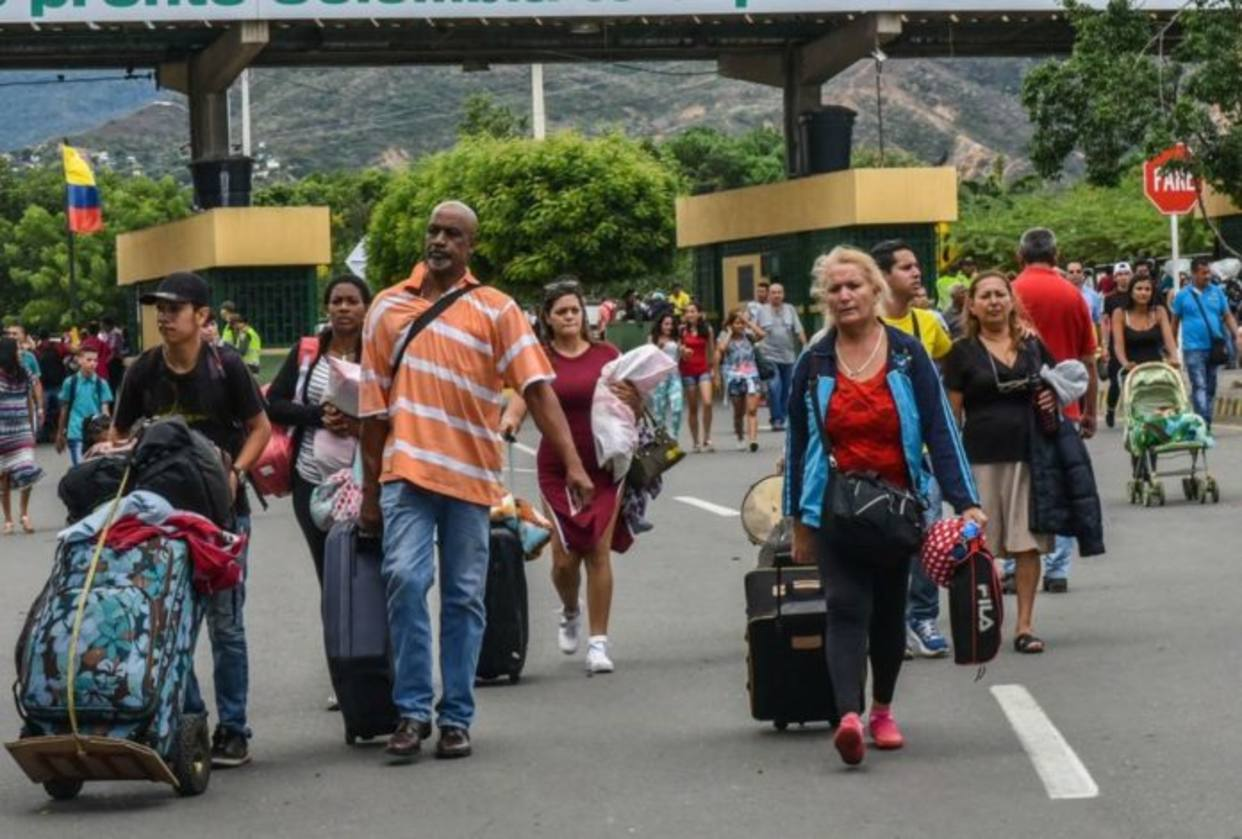
\includegraphics[width=300px]{237.jpg}%
\newline%
%
Aproximadamente 1,9 millones de personas han migrado de Venezuela desde 2015~debido a la situación política y económica que atraviesa el país,~informó un reporte de la Organización de las Naciones Unidas.%
\newline%
%
“Con más de 2,6 millones de personas en el exterior del país actualmente, es crucial una perspectiva apolítica y humanitaria para ayudar a los países que les reciben en un número que va en aumento”, declaró~Filippo Grandi, alto comisionado de la ONU.%
\newline%
%
"Unas 5.000 personas abandonan Venezuela cada día en la actualidad, es el mayor movimiento de población en la historia reciente de América Latina", agregó.%
\newline%
%
"Según los datos oficiales gubernamentales, estimamos que 1,9 millones de venezolanos dejaron su país desde 2015 para dirigirse principalmente hacia otros países de América del Sur como Brasil, Colombia, Ecuador y Perú", explicó William Spindler, portavoz de Acnur a la agencia de noticias~AFP.%
\newline%
%
"El gran éxodo empezó este año, se observaba esta tendencia desde principios de año",~precisó el portavoz.%
\newline%
%
La población venezolana está asfixiada en una crisis económica caracterizada por la hiperinflación, la pobreza, la falta de servicios públicos y la escasez de productos de primera necesidad, especialmente de medicamentos y alimentos. Esto ha provocado un éxodo masivo de cientos de miles de venezolanos.%
\newline%
%
"Felicito a los Estados que han mantenido sus fronteras abiertas y que ofrecen asilo u otras formas de estancia legal a los venezolanos", dijo Grandi. "Todavía queda mucho por hacer para garantizar la coherencia regional de la respuesta aportada en materia de protección~de los individuos", advirtió.%
\newline%
%
\end{document}